\documentclass[main]{subfiles}


\title[AutoML: NAS]{Neural Architecture Search}
\subtitle{How to choose a NAS search space?}
\author[Jovita Lukasik]{Jovita Lukasik}
\date{}

\titlebackground*{images/AutoML_HPO_2_2}

%\institute{}
%\date{}

\begin{document}
	
	\maketitle


\begin{frame}{Search Spaces}
\begin{center}
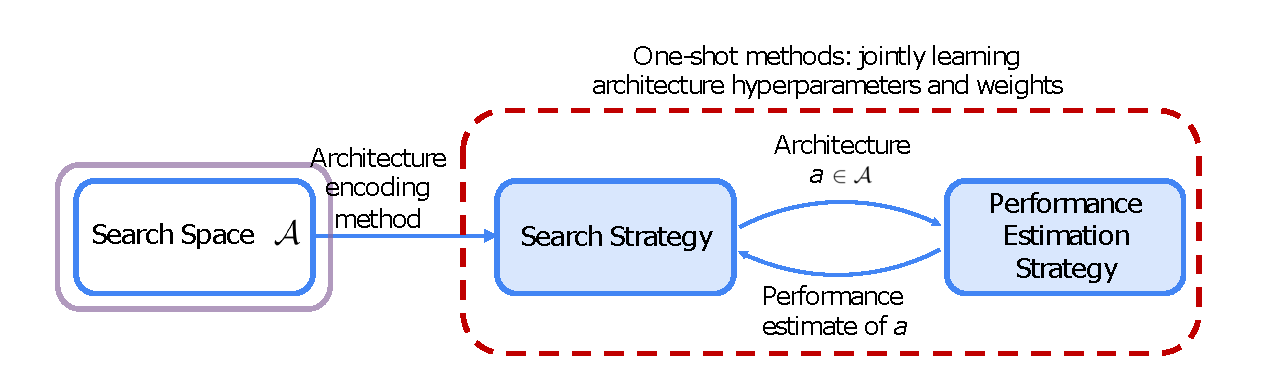
\includegraphics[height=3cm]{images/02/white_2023_nas_overview_1.pdf}
\captionof{figure}{Overview of neural architecture search ~\liturl{White et al. 2023}{https://arxiv.org/pdf/2301.08727.pdf}}
\end{center}
Defining a search space is the first step when setting up NAS
\end{frame}

\begin{frame}{Background on Search Spaces}
\begin{minipage}[c]{0.65\textwidth}
    \begin{center}
    \begin{itemize}
    \item Defining a search space is the first step when setting up NAS
    \item Most human expert knowledge needed here
    \item Majority is task-specific and inspired by manually designed architectures
    \item Main pattern: Repeated blocks \liturl{He et al. 2016}{https://www.cv-foundation.org/openaccess/content_cvpr_2016/papers/He_Deep_Residual_Learning_CVPR_2016_paper.pdf}

\end{itemize}
\end{center}
\end{minipage}
\begin{minipage}[c]{0.1\textwidth}
    \begin{center}
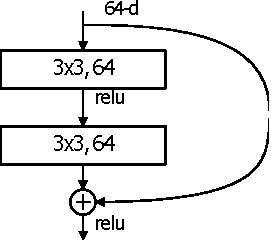
\includegraphics[width=1cm]{images/02/resnet34_block_deeper.pdf}
    \end{center}
\end{minipage}
\begin{minipage}[c]{0.2\textwidth}
    \begin{center}
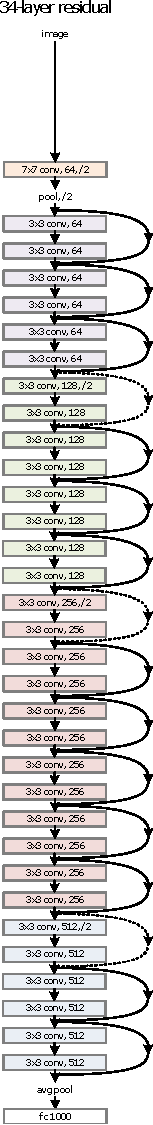
\includegraphics[height=6cm]{images/02/resnet34_arch.pdf}
    \end{center}
\end{minipage}
\end{frame}

\begin{frame}{Overview of Search Space Types}

\begin{table}[t] %[ht!b]
\resizebox{0.8\linewidth}{!}{

\begin{tabular}{@{}lllc@{}}
\toprule
\multicolumn{1}{c}{\textbf{Search Spaces}}  & \multicolumn{1}{c}{\begin{tabular}[c]{@{}c@{}} \textbf{Structure} \end{tabular}} & \multicolumn{1}{c}{\begin{tabular}[c]{@{}c@{}} \textbf{Searchable hyperparameters} \end{tabular}}                                                                 & \begin{tabular}[c]{@{}c@{}} \textbf{Levels of}  \\ \textbf{Topology}\end{tabular}  \\\midrule 
\begin{tabular}[c]{@{}l@{}} \textbf{Macro search space} \\ e.g. NASBOT ~\liturl{Kandasamy et al. 2018}{https://proceedings.neurips.cc/paper_files/paper/2018/file/f33ba15effa5c10e873bf3842afb46a6-Paper.pdf},\\ EfficientNet ~\liturl{Tan and Le 2019}{http://proceedings.mlr.press/v97/tan19a/tan19a.pdf} \end{tabular}  & \begin{tabular}[c]{@{}l@{}} DAG \end{tabular}                                                                                                & \begin{tabular}[c]{@{}l@{}} Operation types, DAG topology, \\ macro hyperparameters \end{tabular} & 1                          \\ \midrule
\begin{tabular}[c]{@{}l@{}} \textbf{Chain-structured search space} \\
e.g. MobileNetV2~\liturl{Sandler et al. 2018}{https://openaccess.thecvf.com/content_cvpr_2018/papers/Sandler_MobileNetV2_Inverted_Residuals_CVPR_2018_paper.pdf}
\end{tabular} & \begin{tabular}[c]{@{}l@{}} Chain \end{tabular}                              & Operation types, macro hyperparameters                                                                                                                                                                & 1                          \\\midrule
\begin{tabular}[c]{@{}l@{}} \textbf{Cell-based search space} \\ e.g. DARTS~\liturl{Liu et al. 2019}{https://openreview.net/pdf?id=S1eYHoC5FX}
\end{tabular}    & Duplicated cells                                                                                           & Operation type, cell topology                                                                                                                                                                   & 1                          \\\midrule
\begin{tabular}[c]{@{}l@{}} \textbf{Hierarchical search space} \\ e.g. Hier. Repr.~\liturl{Liu et al. 2018}{https://openreview.net/pdf?id=BJQRKzbA-}, \\ Auto-DeepLab~\liturl{Liu et al. 2019}{https://openaccess.thecvf.com/content_CVPR_2019/papers/Liu_Auto-DeepLab_Hierarchical_Neural_Architecture_Search_for_Semantic_Image_Segmentation_CVPR_2019_paper.pdf}  \end{tabular} & Varied                                                                                           & \begin{tabular}[c]{@{}l@{}}Operation type, cell/DAG topology, \\ macro hyperparameters \end{tabular} & $>1$ \\ \bottomrule
\end{tabular}}

\caption{Summary of the types of NAS search spaces ~\liturl{White et al. 2023}{https://arxiv.org/pdf/2301.08727.pdf}.
\label{tab:search_space_summary}
}
\end{table}
    
\end{frame}

\begin{frame}{Basic Search Spaces}
\begin{itemize}
    \item Macro search space
    \item Chain-structured search space
    \item More complex search spaces
\end{itemize}  
\end{frame}

\begin{frame}{Macro Search Spaces}
\begin{itemize}
    \item Two types:
    \begin{enumerate}
        \item Encode entire architecture
        \item Variation of macro-level hyperparameters, e.g., where and how much to downsample
    \end{enumerate}
\end{itemize}

\begin{minipage}[c]{0.3\textwidth}
    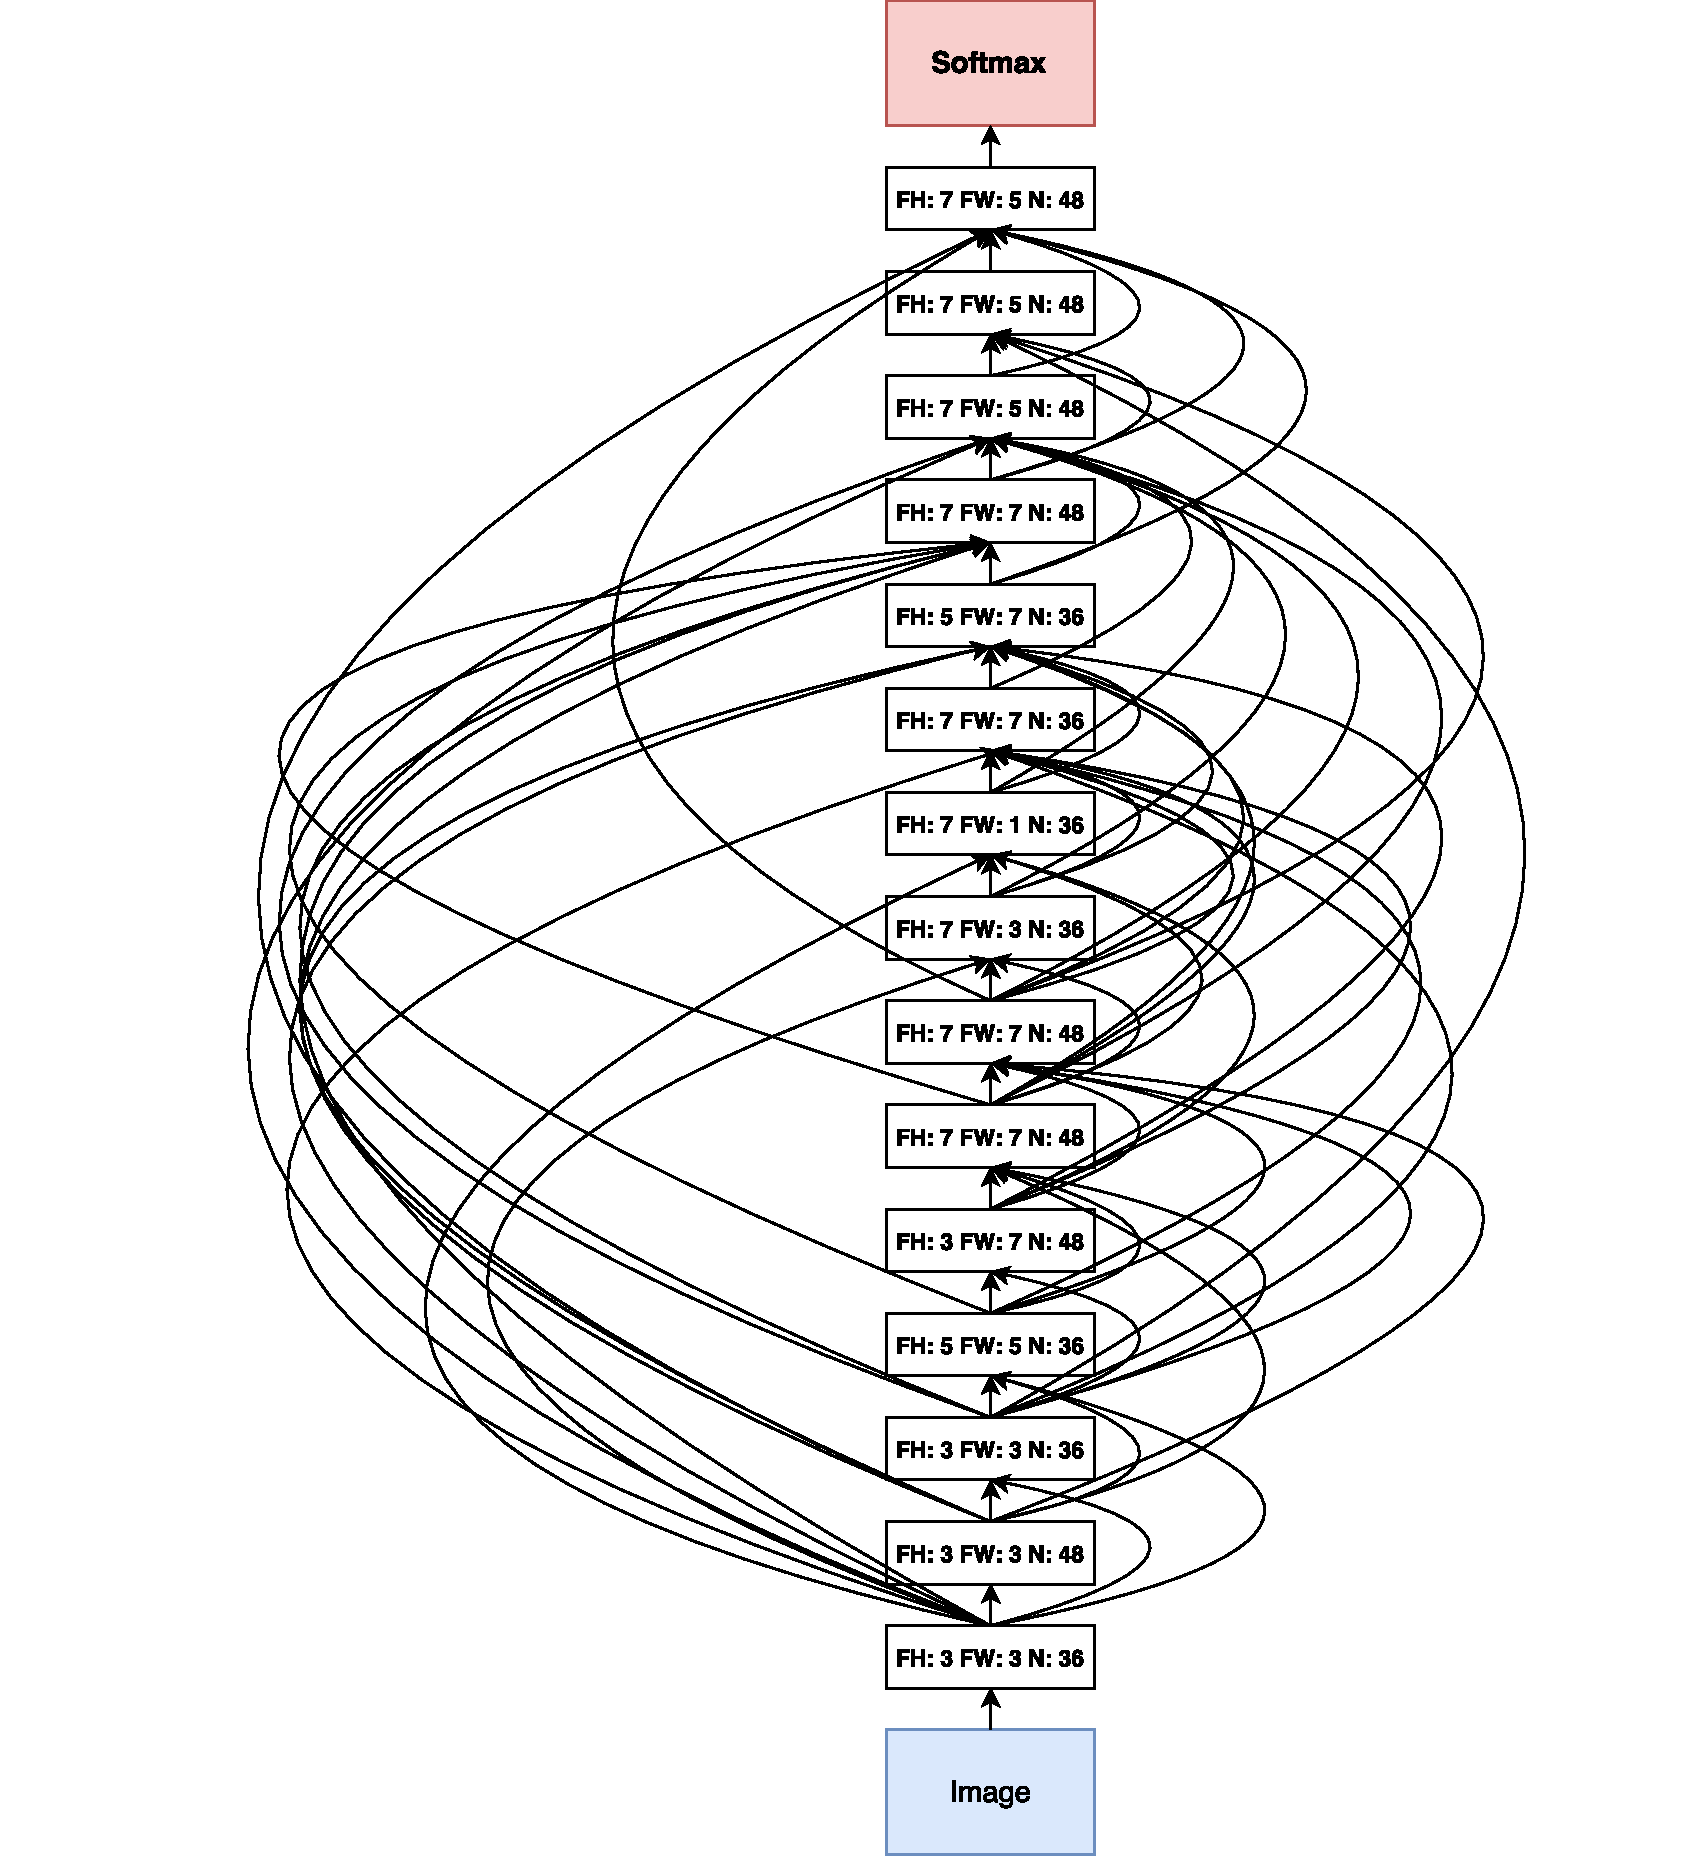
\includegraphics[height=5cm]{images/02/Conv_Structure.pdf}
    \captionof{figure}{Example of an entire architecture encoding ~\liturl{Zoph and Le 2017}{https://openreview.net/pdf?id=r1Ue8Hcxg}}
\end{minipage}
\begin{minipage}[c]{0.65\textwidth}
        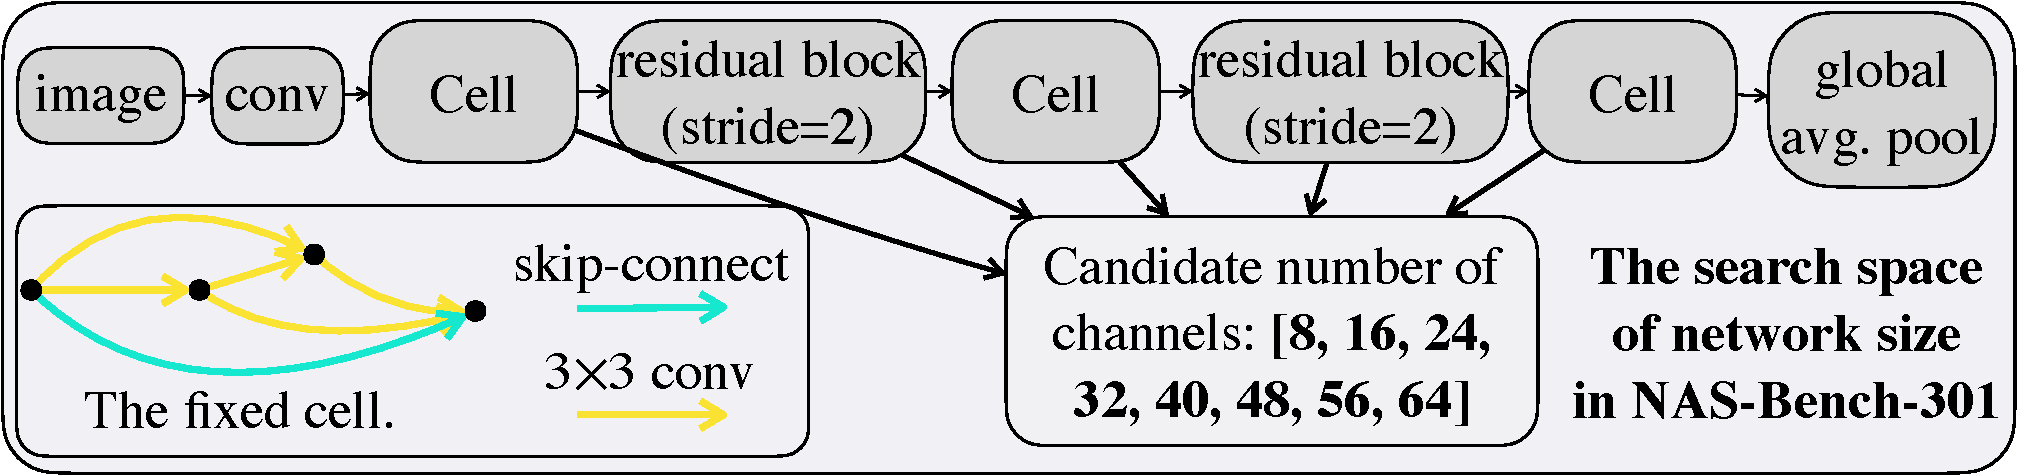
\includegraphics[height=2cm]{images/02/size-search-space.pdf}
    \captionof{figure}{Example of macro-level hyperparameters~\liturl{Dong et al. 2021}{https://ieeexplore.ieee.org/stamp/stamp.jsp?tp=&arnumber=9336247}}
\end{minipage}
\end{frame}
\begin{frame}{Marco Search Spaces}
Pros:
\begin{itemize}
    \item High representation power
    \item Flexible structure allows for discovering novel architectures
\end{itemize}
Cons:
\begin{itemize}
    \item Very slow to search
\end{itemize}
    
\end{frame}

\begin{frame}{Chain-structured Search Spaces}
\begin{itemize}
    \item Chain-structured search space are the most basic variant of search spaces. 
    \item Can be easily adapted to multi-brach networks
    \begin{itemize}
        \item More degrees of freedom
    \end{itemize}
\end{itemize}

\begin{minipage}[c]{0.45\textwidth}
\centering
    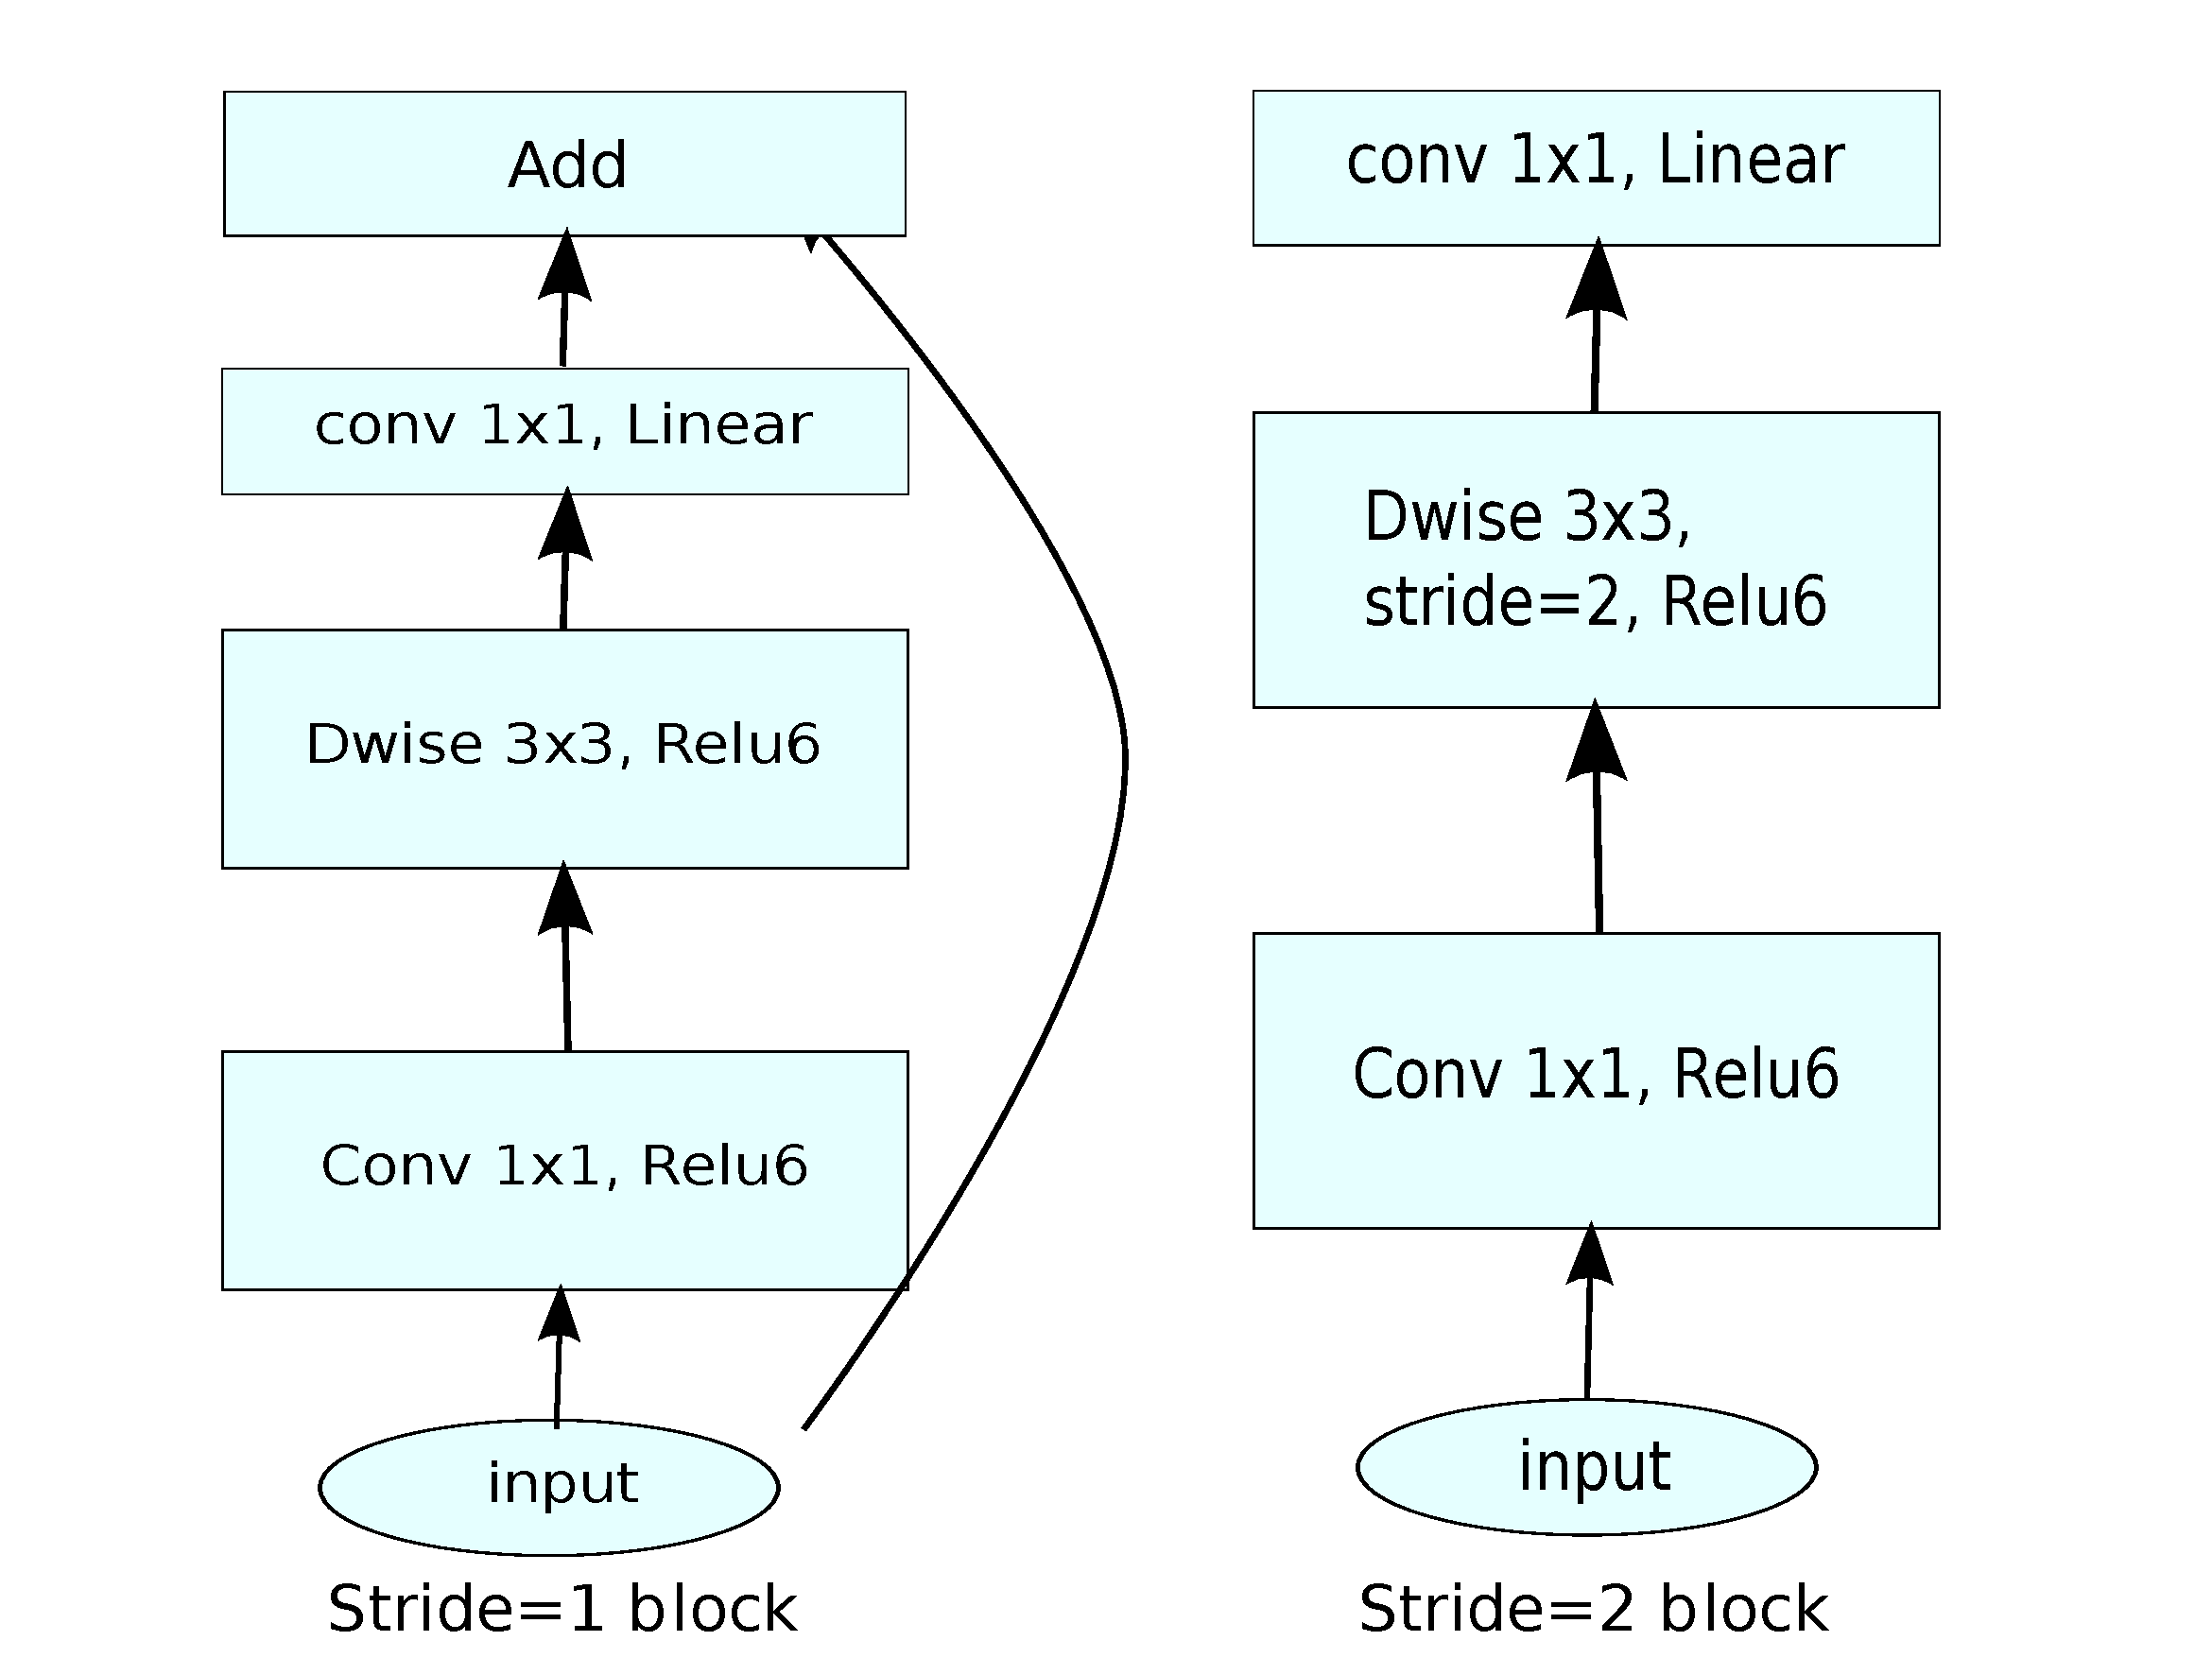
\includegraphics[height=3cm]{images/02/mobilenet_v2_block.pdf}
    \captionof{figure}{Convolution blocks in MobileNet V2 ~\liturl{Sandler et al. 2018}{https://openaccess.thecvf.com/content_cvpr_2018/papers/Sandler_MobileNetV2_Inverted_Residuals_CVPR_2018_paper.pdf}}
\end{minipage}
\begin{minipage}[c]{0.45\textwidth}
\centering
        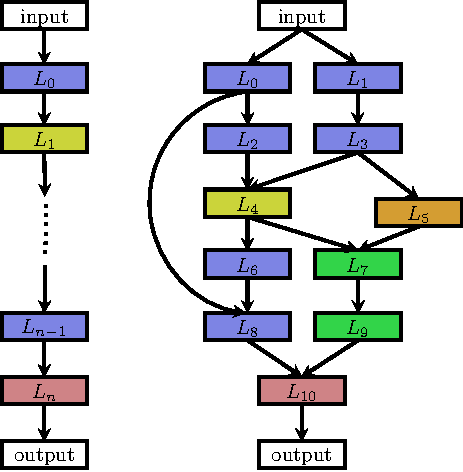
\includegraphics[height=3cm]{images/02/chain_mb_space_v2.pdf}
    \captionof{figure}{left: Example of chain-structured search space. right: More complex search space with multiple branches. \liturl{Elksen et al. 2019}{https://www.jmlr.org/papers/volume20/18-598/18-598.pdf}}
\end{minipage}   
\end{frame}

\begin{frame}{Cell-based Search Spaces}
\begin{minipage}[c]{0.45\textwidth}
\begin{itemize}
    \item Most popular search space in NAS
    \item Inspired by repetitive block in human designed CNNs (e.g., ResNet blocks \liturl{He et al. 2016}{https://www.cv-foundation.org/openaccess/content_cvpr_2016/papers/He_Deep_Residual_Learning_CVPR_2016_paper.pdf})
    \item Start with NASNet~\liturl{Zoph et al. 2018}{https://openaccess.thecvf.com/content_cvpr_2018/papers/Zoph_Learning_Transferable_Architectures_CVPR_2018_paper.pdf}: Search for small cells and stack them several times (i.e., micro strucutre with fixed marco architecture)
    \item Different types of cells used: normal and reduction cell (same structure with different strides)
        
\end{itemize}
\end{minipage}
\begin{minipage}[c]{0.45\textwidth}
\centering
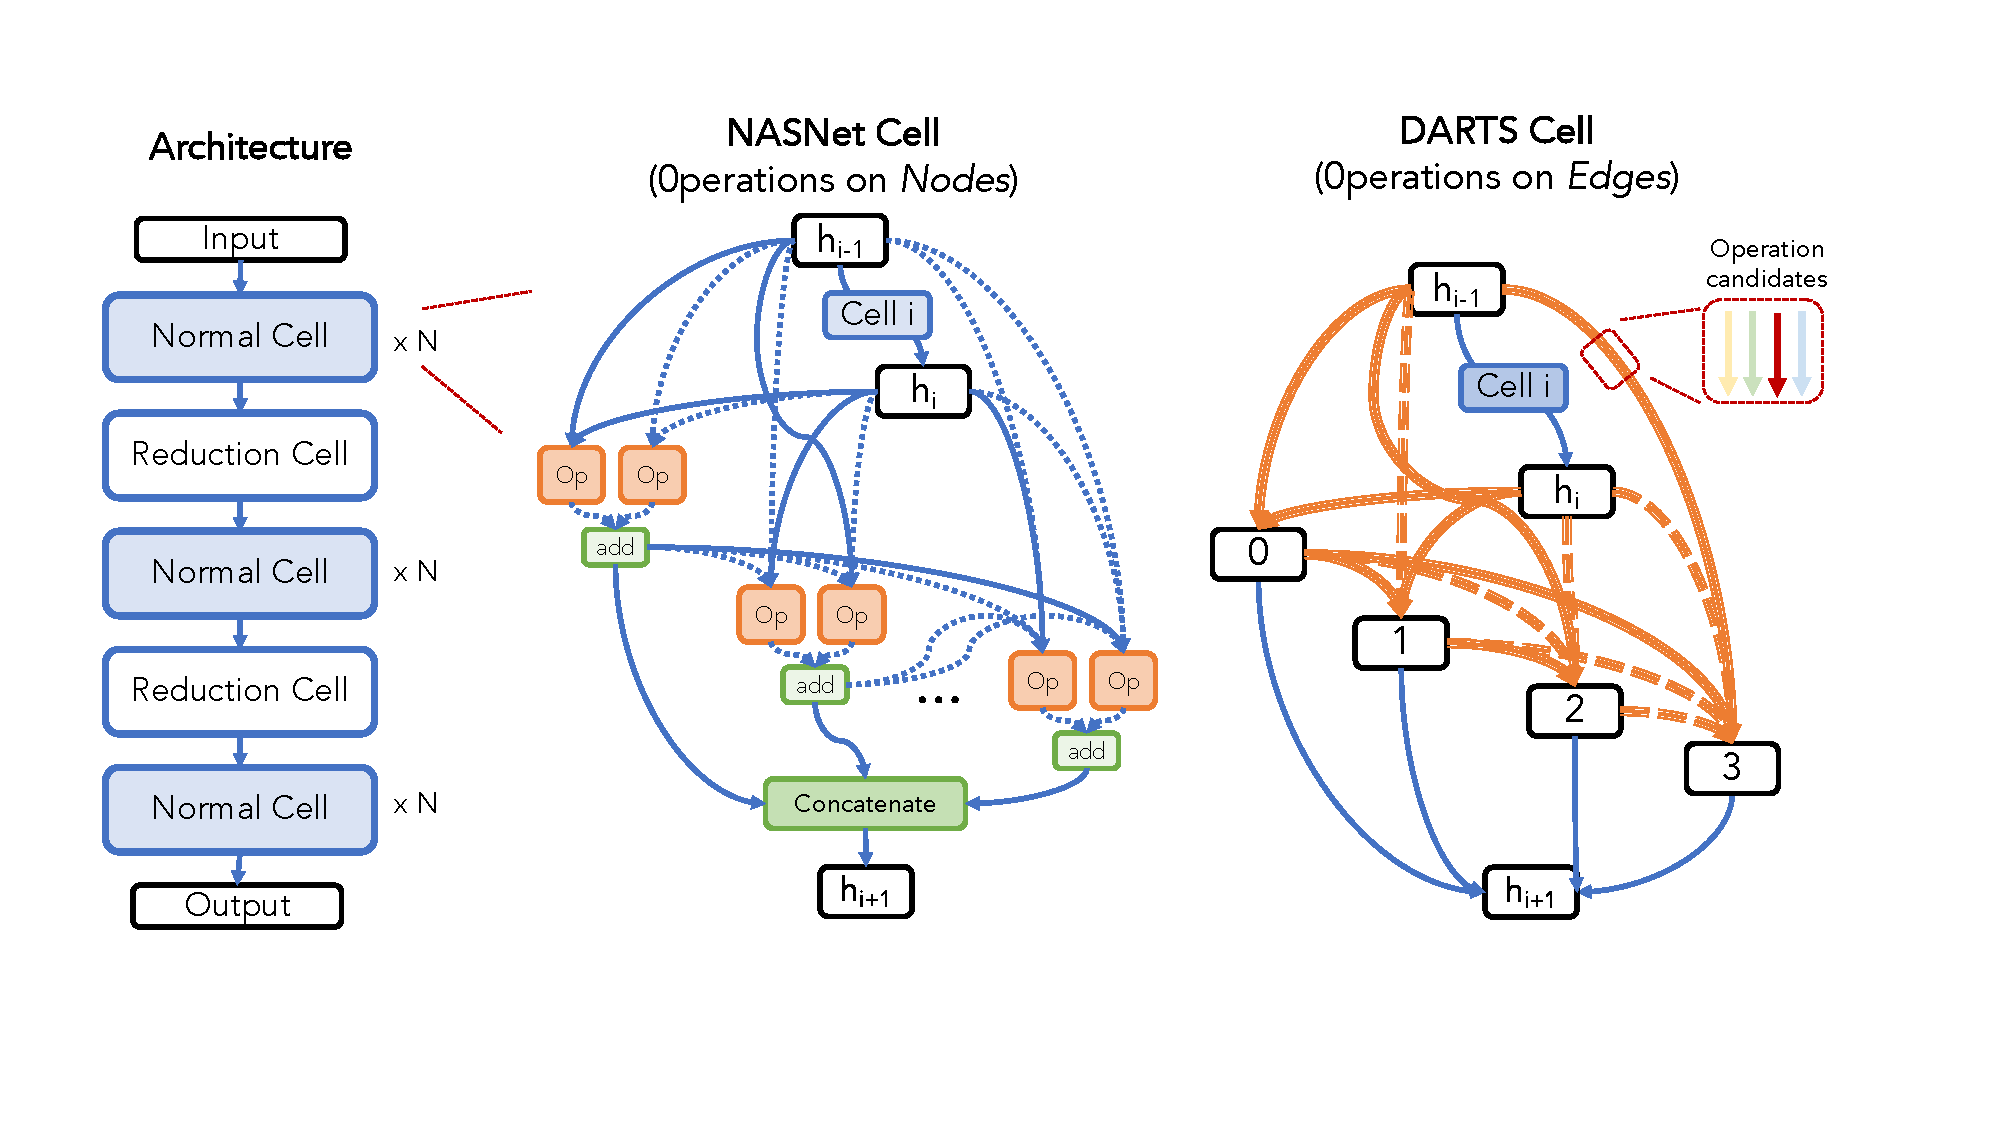
\includegraphics[width=6cm]{images/02/cell_ss2.pdf}
    \captionof{figure}{Visualization of different cell-based search spaces~\liturl{White et al. 2023}{https://arxiv.org/pdf/2301.08727.pdf}}
\end{minipage}
    
\end{frame}

\begin{frame}{Cell-based Search Spaces}
\alert{NASNet}~\liturl{Zoph et al. 2018}{https://openaccess.thecvf.com/content_cvpr_2018/papers/Zoph_Learning_Transferable_Architectures_CVPR_2018_paper.pdf}
\begin{itemize}
    \item Search for blocks (i.e., cells) with 5 choices
    \begin{itemize}
        \item Choose 2 previous feauture maps
        \item Choose operations for both (convolutions, pooling)
        \item Choose operation to merge (add or concat)
    \end{itemize}
\end{itemize}
\begin{center}
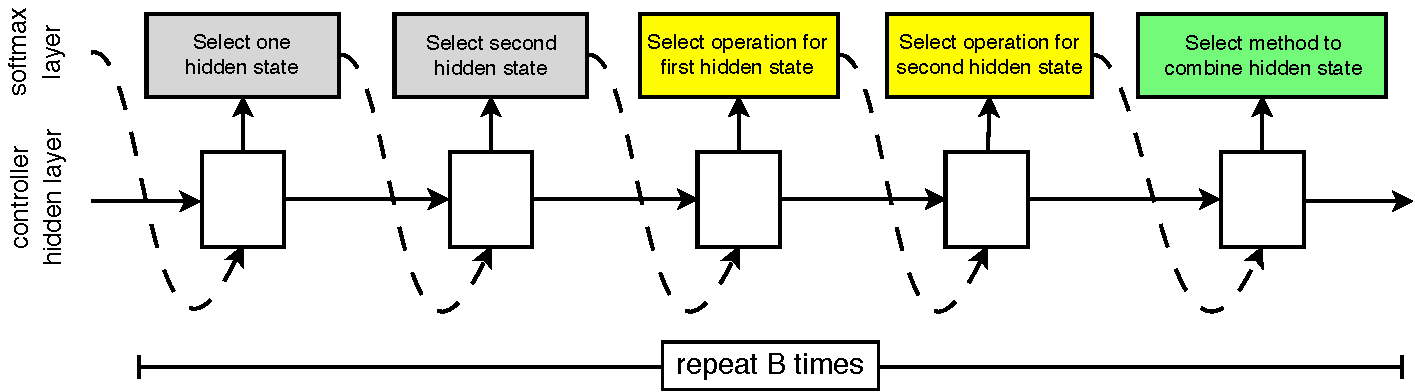
\includegraphics[height=2.5cm]{images/02/nasnet_Figure-2.pdf}
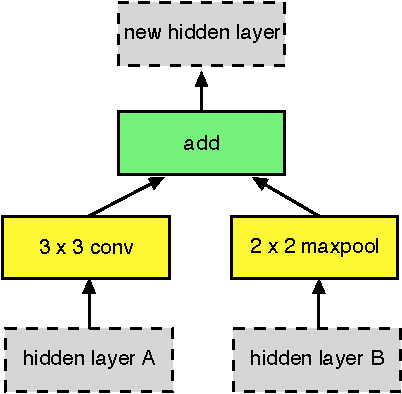
\includegraphics[width=2.5cm]{images/02/nasnet_Figure-2-Part-B.pdf}
  \captionof{figure}{Visualization of one block construction in NASNet search space.}
\end{center}
\end{frame}

\begin{frame}{Cell-based Search Spaces}
Pros:
\begin{itemize}
    \item Reduces  search space size
    \item Transferability to other datasets (cells from CIFAR-10 to ImageNet)
    \item Stacking pattern based on human knowledge as has shown superior performance
\end{itemize}

Cons:
\begin{itemize}
    \item Manual design of macro architecture 
    \item Limiting, if search for one cell, which is repeatedly stacked 
    \item Ad-hoc design choices have unclear impact
    \item Search space less expressive
    \item Possible low variance of performance of architectures
\end{itemize}
\end{frame}

\begin{frame}{Hierarchical Search Spaces}
\begin{itemize}
    \item Design motifs at different levels 
    \item Each higher-level motif represented as directed acyclic graph of lower-level motifs
    \item Different level of motifs ~\liturl{Liu et al. 2018}{https://openreview.net/pdf?id=BJQRKzbA-}:
    \begin{itemize}
        \item Level 1 operation primitives, such as $3\times 3$ convolutions, average pooling
        \item Level 2 motifs combines level 1 operation primitives
        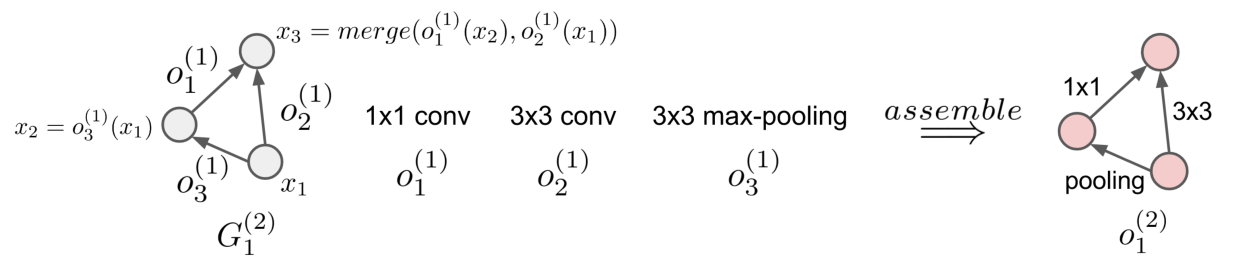
\includegraphics[height=1.5cm]{images/02/hier_level_2.png}
        \item Level 3 motifs combines level 2 motifs
        
         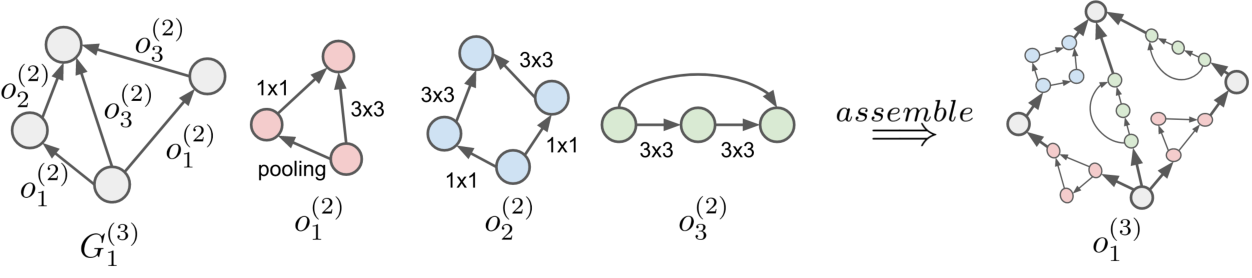
\includegraphics[height=1.5cm]{images/02/hier_level_3.png}
    \end{itemize}
\end{itemize}
\end{frame}

\begin{frame}{Hierarchical Search Spaces}
Pros:
\begin{itemize}
    \item More expressive
    \item Flexibility of constructing building blocks (as in cell-based search spaces) 
    \item Flexibility of different building blocks (as in basic search spaces)
    \item Reuse building blocks at various levels 
    \item Reduce search complexity by hierarchical representation of large architecture 
\end{itemize}
Cons:
\begin{itemize}
    \item Larger than cell-based search space
    \item More expresive which can lead to potentail harder search
\end{itemize}
\end{frame}
%----------------------------------------------------------------------
\begin{frame}{Summary} 

Most important insights from this video:

\begin{enumerate}
    \item ???
    \item ???
    \item ???
\end{enumerate}


\end{frame}



\end{document}
